\section{Approach}

\subsection{Overview}

To test the DFR tools, we first designed hypothetical test scenarios involving factors which would make recovery difficult. We then created each scenario in real filesystems and saved them as raw images. Using the images as input, we ran each DFR tool and attempted to recover all deleted files. Finally, we compared the recovered files to their original versions in order to judge the tools' compliance with the NIST standards.  \ref{fig:overview}

\begin{figure}[h]
    \centering
    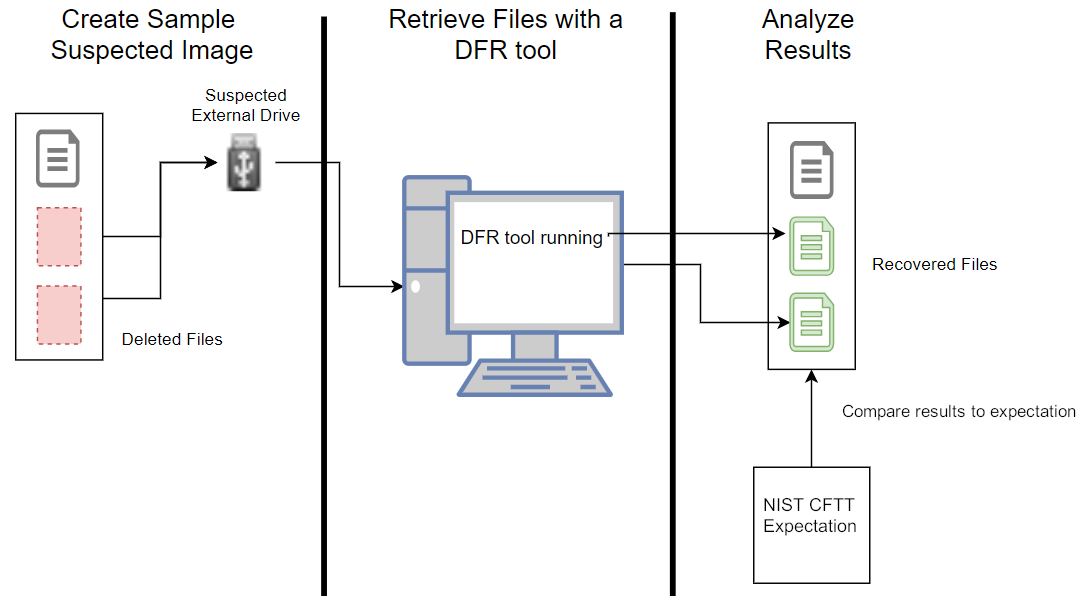
\includegraphics[width=\linewidth]{fig/overview.png}
    \caption{The DFR tool targets to retrieve deleted files. The recovery accuracy is compared to the NIST CFTT standard.}
    \label{fig:overview}
\end{figure}

\subsection{Designing Recovery Scenarios}
To test the DFR tools' compliance with the standards, we designed a variety of scenarios in which a tool might have to recover a deleted file. We started with the simplest possible case: a filesystem containing just one deleted file. This case is ideal and trivial, but by adding more files, we can create far more complex scenarios.

% Fragmentation and Overwriting are the two things that can complicate file recovery 
The NIST standards limit the scope of testing to situations in which files were ``created and deleted in a process similar to how an end-user would create and delete files,''\cite{meta:dfr:standards} and  exclude ``files and file system metadata that is specifically corrupted, modified, or otherwise manipulated to appear deleted.''\cite{meta:dfr:standards}
Within these constraints, there are two factors which can significantly complicate the file recovery process: fragmentation, and overwriting. \comment{need to make sure these are defined elsewhere, if not they should be defined here}

% Make different varieties of Fragmentation and overwriting, and combinations
These factors are thus the focus of our test scenarios, with all cases besides the first involving either fragmented files, overwritten files, or a combination of both.

We designed the following test cases:
\begin{itemize}
    \item [1] Single deleted file
    \item [2] Deleted file fragmented around an active file\ref{fig:case_2}
    \begin{figure}[h]
        \centering
        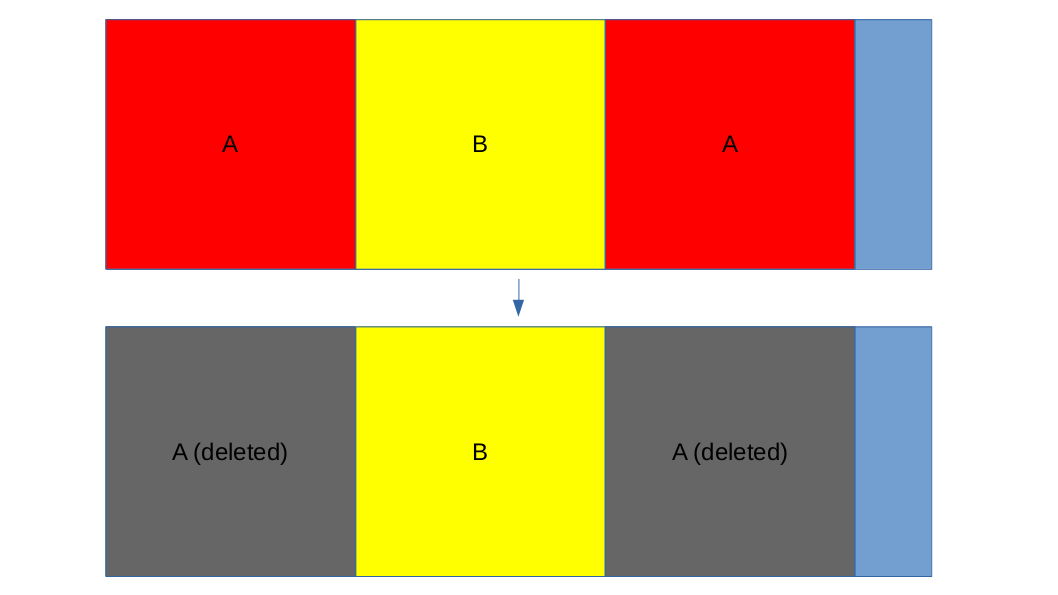
\includegraphics[width=\linewidth]{fig/case2.png}
        \caption{Test Case 2}
        \label{fig:case_2}
    \end{figure}
    \item [3]
 Deleted file fragmented around a deleted file
    \item [4i]
 Beginning of deleted file overwritten by an active file\ref{fig:case_4i}
    \item [4ii]
 Middle of deleted file overwritten by an active file
        \begin{figure}[h]
        \centering
        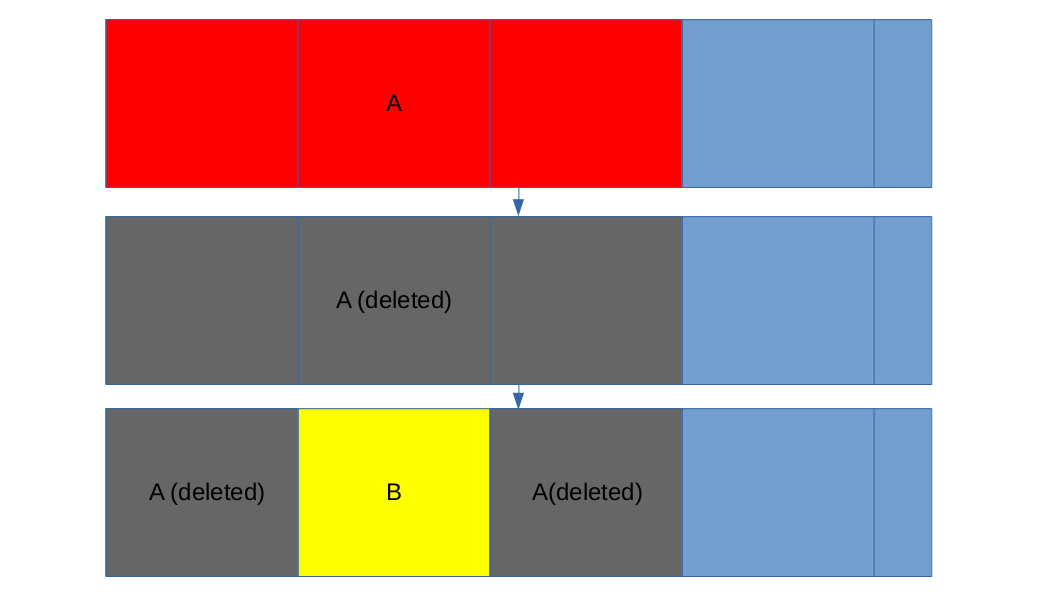
\includegraphics[width=\linewidth]{fig/case4ii.png}
        \caption{Test Case 4ii}
        \label{fig:case_4ii}
    \end{figure}
    \item [4iii]
 Deleted file partially overwritten by an active file which doesn't end on a sector boundary
    \item [4iv]
 Deleted file entirely overwritten by an active file
    \item [5i]
 Beginning of deleted file overwritten by a deleted file
    \item [5ii]
 Middle of deleted file overwritten by a deleted file
    \item [5iii]

 Deleted file partially overwritten by a deleted file which doesn't end on a sector boundary
    \item [5iv]
 Deleted file entirely overwritten by a deleted file
    \item [6]
 Deleted file fragmented around an active file, with the second fragment overwritten by an active file\ref{fig:case_6}
    \begin{figure}[h]
        \centering
        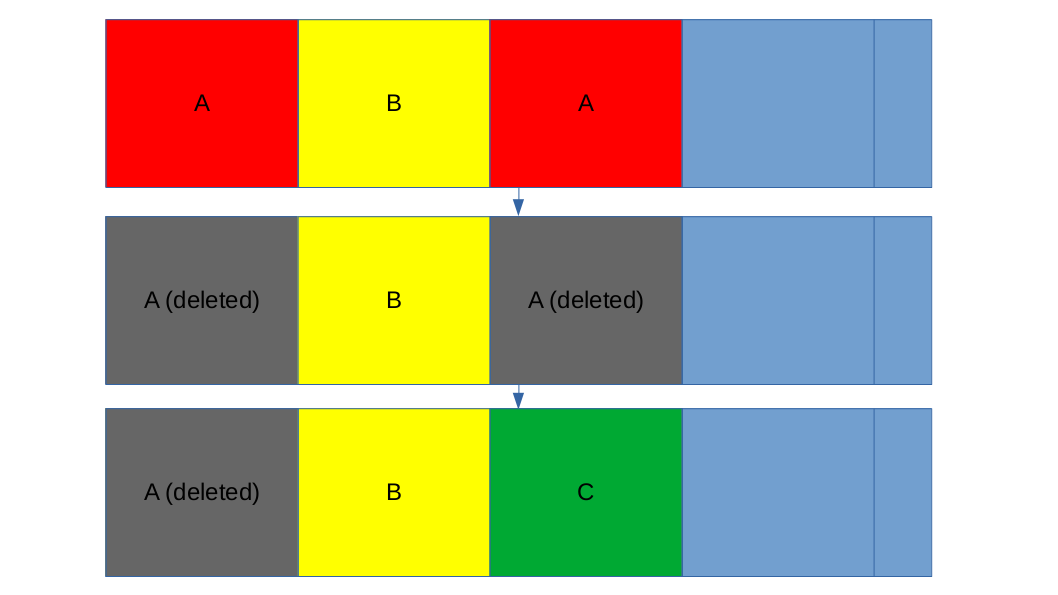
\includegraphics[width=\linewidth]{fig/case6.png}
        \caption{Test Case 6}
        \label{fig:case_6}
    \end{figure}
    \item [7]
 Deleted file fragmented around an active file, with the second fragment overwritten by a deleted file
    \item [8]
 Deleted file fragmented from the end of the filesystem to the beginning
    \item [9]
 Deleted file fragmented from the end of the filesystem to after an active file
    \item [10]
 Deleted file fragmented from the end of the filesystem to after a deleted file
\end{itemize}

Because NTFS keeps track of the locations of all parts of a file even after deletion, fragmentation is not particularly interesting. Cases 8, 9, and 10 would be redundant with case 2, so we have excluded them for NTFS. Due to how NTFS allocates space for files, cases 4ii and 5ii cannot occur as a result of normal file operations, so they have also been excluded. No cases are excluded for FAT tests.

\subsection{Creating Test Images}
% Step by step process
All test filesystems were created in partitions on a 32 GB flash drive. For each test case, the first step is to entirely write over the partition with zeros. This ensures all cases start from identical, reproduceable conditions. A new filesystem is written to the partition, then new files are written to the filesystem and deleted. The files used are simple text files containing one letter repeated (e.g. ``aa1M'' is 1 MiB of the letter 'a'). Files are written to the test filesystem by simply copying them from another drive. In some cases we also append data to a file in the test filesystem. Once the test filesystem matches the intended scenario, a read-only image of the partition is created. All tests are performed on these images rather than the original drive.

% Caching problem
It is important to consider when creating test images that the low-level behavior of file operations is not always obvious. For example, when writing a file, there is no guarantee the file's data will be immediately written to the disk. The operating system may cache the operation and wait until the optimal time to perform the write, in order to maximize system performance. We observed this early on, as writing a file and subsequently deleting it would always result in the file's metadata being written, but often left no evidence of the file's data having ever existed. This behavior is obviously undesireable because it leaves nothing meaningful to be recovered. We resolved this by calling the ``sync'' system call, which causes any such cached data to be immediately written to the disk, in between file writes and deletions. Unmounting the filesystem has a similar effect.

% Learning and using the allocation algorithms
Another type of low-level behavior relevant to the image creation process is the allocation algorithm. The operating system must have some kind of algorithm to decide where in the data area new files should be written. Common allocation algorithms include ``first available,'' ``next available,'' and ``best fit.'' %TODO cite
Learning and understanding whatever algorithm the OS uses is very helpful for forcing a specific arrangement of files. We observed that when writing to a FAT filesystem, Linux uses a ``next available'' algorithm. After the filesystem is mounted, the first write will start at the first free space in the data area. The next file will be written starting from the first free space after the previous file.
Meanwhile, when writing to an NTFS filesystem, Windows 10 appears to use a ``best fit'' algorithm. In this case, Windows tries to find the smallest space in which the file can fit without being fragmented, and write it there.

% Directory entries problem

\subsection{Recovering Files}

When testing Autopsy, we performed a standard recovery with all ingest modules disabled.
For Recuva we perfomed a standard recovery using the free version with no settings altered.
\comment{what settings did we use for FTK?}
For TestDisk we used the ``file undelete'' feature under ``Advanced Filesystem Utils.''
For Magnet Axiom we performed a ``full scan'' using the full version of the software. Magnet Axiom was tested on a separate set of filesystem images; the original images contained text files with no file extension, which Magnet Axiom did not identify. We remade the images, adding the ``.txt'' extension to all files, and tested Magnet Axiom with the new images.

\subsection{Results}

After testing each tool, we analyzed the recovered object(s) from each test case. If the recovered file is identical to the original, obviously all standards have been met. However, this only ever occurred for FAT cases 1 and 2, and NTFS cases 1-3. In all other cases, the tool is judged on each core feature individually. These judgements are summarized in the figure.\ref{fig:results}

\begin{figure}[h!]
    \centering

    \begin{subfigure}{0.3\linewidth}
        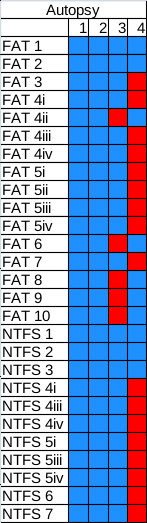
\includegraphics[width=\linewidth]{fig/autopsy_results.png}
        \subcaption{Autopsy}
    \end{subfigure}
    ~
    \begin{subfigure}{0.3\linewidth}
        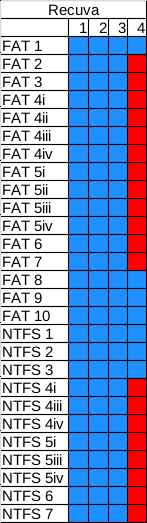
\includegraphics[width=\linewidth]{fig/recuva_results.png}
        \subcaption{Recuva}
    \end{subfigure}
    ~
    \begin{subfigure}{0.3\linewidth}
        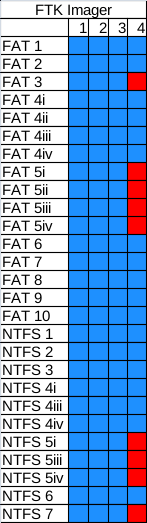
\includegraphics[width=\linewidth]{fig/ftk_results.png}
        \subcaption{FTK}
    \end{subfigure}
    
    
    \begin{subfigure}{0.3\linewidth}
        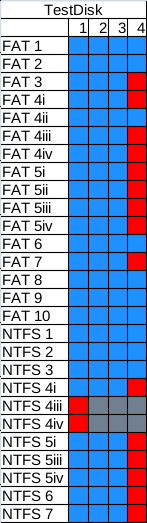
\includegraphics[width=\linewidth]{fig/testdisk_results.png}
        \subcaption{TestDisk}
    \end{subfigure}
    ~
    \begin{subfigure}{0.3\linewidth}
        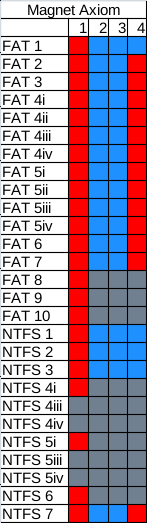
\includegraphics[width=\linewidth]{fig/axiom_results.png}
        \subcaption{Magnet Axiom}
    \end{subfigure}
        
    \caption{Test results organized by tool. Rows represent test cases while columns represent NIST core features. Blue is passing, red is failing, grey is not tested.}
    \label{fig:results}
\end{figure}

For cases in which a tool does not fulfull core feature 1, in other works, it cannot find a deleted file, we make no judgement about the remaining core features. An exception is made for Magnet Axiom, which we found does not identify certain files (text files without an extension), but can in most cases identify them when they are renamed. We consider Magnet Axiom failing to fulfill core feature 1 for all cases, and make our judgements about the other core features based on a separate set of images with renamed files. Results for NTFS cases 4iii, 4iv, 5iii, and 5iv have been excluded due to errors in the alternate test images for those cases.

In cases of fragmentation in FAT filesystems, we found each tool generally approaches recovery in one of two ways. Recuva and Magnet Axiom start from the beginning of the file and recover the full length of the file even if an active file exists in that space. Autopsy, FTK, and TestDisk will start from the beginning of the file and recover the full length, but skip over any active files they encounter. This can be seen in the results\ref{fig:results} for FAT case 2\ref{fig:case_2}. Autopsy, FTK, and TestDisk recover all of file A, while Recuva and Magnet Axiom's recovered images erroneously contain data from file B, causing them to fail core feature 4. When the space in between fragments is unallocated, all tools recover the file as though it was contiguous, pulling some erroneous data and failing core feature 4. When the fragmentation occurs at the end of the filesystem, Recuva, FTK, and TestDisk recover only the first fragment, while Autopsy returns a short file of null data, and Magnet Axiom does not identify a deleted file at all. Cases with fragmentation are trivial for NTFS filesystems as more metadata is available. Unsurprisingly, no tools had problems with fragmentation cases for NTFS.

In cases where a file has been overwritten by an active file, we found most tools recover the deleted file as though it is not overwritten, failing core feature 4. The exceptions are FTK Imager, which recovers the file up to the point where it has been overwritten, and Autopsy, which generally recovers only the first cluster of an overwritten file in FAT, and behaves like the other tools for NTFS. TestDisk also exhibits the same behavior as FTK for FAT case 4ii only. When the overwriting file has also been deleted, all tools recover the first file as though it is not overwritten.

A few results stand out as unusual. For FAT cases 4ii, 6, 8, 9, and 10, Autopsy returns a 1.5 KiB file of null data. 1.5 KiB is equivalent to 3 sectors; a FAT cluster in our cases is equivalent to 4 sectors or 2 KiB.
TestDisk fails to find a file for NTFS cases 4iii and 4iv only. Besides Magnet Axiom, these are the only test cases in which a tool does not fulfill core feature 1.

% Explain Magnet Axiom filenames issue
